%%%%%%%%%%%%%%%%%%%%%%%%%%%%%%%%%%%%%%%%%%%%%%%%%%%%%%%%%%%%%%%%%%%%%%%%%%%%%
% Chapter 1: Introducci�n 
%%%%%%%%%%%%%%%%%%%%%%%%%%%%%%%%%%%%%%%%%%%%%%%%%%%%%%%%%%%%%%%%%%%%%%%%%%%%%%%

%---------------------------------------------------------------------------------
\section{Secci�n Uno}
\label{1:sec:1}

Todo empez� con un hilo en el foro de internet ``forocoches.com'', en �l hablaban de 
que la programaci�n funcional iba a tener cada d�a m�s relevancia porque cuenta con ventajas de 
las cuales la imperativa carece.\\

A ra�z de ello, me interes� por este paradigma y empec� a (e incluso termin� de) leer numerosos 
libros sobre el lenguaje y la programaci�n funcional en general, y a crear peque�os programas en 
Haskell. Haskell es muy interesante debido a que es el lenguaje con mayor nivel de 
abstracci�n en el que he programado hasta hoy.\\

Haskell es id�neo para crear lenguajes de dominio espec�fico. En otras palabras, antes de 
escribir un compilador se captura el lenguaje a compilar (el lenguaje fuente) en un 
tipo. Las expresiones de ese tipo representar�n t�rminos en el lenguaje fuente y normalmente son 
bastante similares al mismo, a pesar de ser, realmente, tipos de Haskell.\\

Luego se representa el lenguaje objetivo como otro tipo m�s. Finalmente, el compilador es 
realmente una funci�n del tipo fuente al tipo objetivo y las traducciones son f�ciles de escribir y 
leer. Las optimizaciones tambi�n son funciones como cualquier otra (ya que realmente en Haskell 
todo es una funci�n, y adem�s, currificada) que mapean del dominio del lenguaje fuente al codominio
del lenguaje objetivo.\\

Por ello los lenguajes funcionales con sintaxis ligera y un fuerte sistema de tipos se consideran 
muy adecuados para crear compiladores y muchas otras cosas cuya finalidad es la traducci�n.\\

Adem�s, Haskell cuenta con mecanismos de abstracci�n muy fuertes que permiten escribir c�digos 
escuetos que se comportan muy bien, como por ejemplo:\\

\begin{itemize}
  \item reconocimiento de patrones
  \item tipos de datos algebraicos (generalizados o no)
  \item lambdas (y por ello, m�nadas)
  \item plegados de listas
\end{itemize}

%---------------------------------------------------------------------------------
\section{Secci�n Dos}
\label{1:sec:2}

\begin{itemize}
  \item Item 1
  \item Item 2
  \item Item 3
\end{itemize}

%---------------------------------------------------------------------------------
\section{Secci�n Tres}
\label{1:sec:3}

Bla, bla, bla

%---------------------------------------------------------------------------------
\section{Secci�n Cuatro}
\label{1:sec:4}

Bla, bla, bla

%------------------------------------------------------------------------------
\begin{figure}[!th]
\begin{center}
\includegraphics[width=0.5\textwidth]{images/arbolbinario.eps}
\caption{Ejemplo}
\label{fig:ArbolBinario}
\end{center}
\end{figure}
%------------------------------------------------------------------------------

